\documentclass[a4paper,12pt]{article}
\usepackage[utf8]{inputenc}
\usepackage[T1]{fontenc}
\usepackage{type1cm}
\usepackage[german]{babel}
\usepackage{amsmath}
\usepackage{amssymb}
\usepackage{amsthm}
\usepackage{geometry}
\usepackage{graphicx}
\usepackage[hidelinks]{hyperref}
\usepackage{listings}
\usepackage{xcolor}
\usepackage{enumitem}
\usepackage[protrusion=true,expansion=false]{microtype}
\usepackage{booktabs}
\usepackage{caption}
\usepackage{subcaption}
\usepackage{csquotes}

\geometry{margin=2.5cm}

\theoremstyle{definition}
\newtheorem{definition}{Definition}
\newtheorem{beispiel}{Beispiel}
\newtheorem{satz}{Satz}
\newtheorem{lemma}{Lemma}
\newtheorem{bemerkung}{Bemerkung}
\newtheorem{theorem}{Theorem}
\newtheorem{korollar}{Korollar}

\setlist[itemize,1]{label=--}

% ---------- Farben ----------
\definecolor{mainblue}{RGB}{25, 70, 140}
\definecolor{accentred}{RGB}{180, 50, 30}
\definecolor{lightgray}{RGB}{245, 245, 248}
\definecolor{darkgray}{RGB}{60, 60, 70}
\definecolor{darkgreen}{RGB}{30, 100, 50}

\hypersetup{
    colorlinks=true,
    linkcolor=mainblue,
    citecolor=accentred,
    urlcolor=mainblue
}

\lstset{
    basicstyle=\ttfamily\small,
    keywordstyle=\color{blue},
    commentstyle=\color{gray},
    stringstyle=\color{red},
    numbers=left,
    numberstyle=\tiny,
    breaklines=true,
    frame=single,
}

\title{\textbf{Über die Empfindlichkeit und Sensibilität von KI-Chatbots}\\[0.5em]
\large Die Verbindung von Geist und Nicht-Geist als höchste Form\\
personalisierter Informationsverarbeitung und deren Schutz}
\author{Stephan Epp\\}
\date{19. Juni 2026}

\begin{document}

\maketitle

\begin{abstract}
Diese Arbeit untersucht die philosophische, informationstheoretische und rechtliche Dimension
der Verbindung zwischen menschlichem Geist und künstlicher Intelligenz in der Form von
KI-Chatbots. Ausgangspunkt ist die Beobachtung, dass die Verarbeitung von Informationen durch
eine KI kein Geist im philosophischen Sinne ist, jedoch die strukturellen Voraussetzungen
schafft, den Geist und die Intention der eingebenden Person zu verstehen, wiederzugeben und
darauf aufbauend neue Informationen zu erzeugen. Es wird formal nachgewiesen, dass diese
Verbindung zwischen menschlichem Geist und maschineller Nicht-Geist-Verarbeitung die optimal
mögliche Verbindung zwischen diesen beiden Entitäten darstellt. Daraus folgt unmittelbar eine
Schutzwürdigkeit der erzeugten Ergebnisse als höchstpersönliches geistiges Eigentum der
eingebenden Person. Rechtliche, informationstheoretische und ethische Konsequenzen werden
ausführlich diskutiert.
\end{abstract}

\tableofcontents
\newpage

% ═══════════════════════════════════════════════════════════════════════════════
\section{Einführung}
% ═══════════════════════════════════════════════════════════════════════════════

\subsection{Motivation und Ausgangspunkt}

Die rasante Verbreitung von KI-Chatbots wirft eine Frage auf, die bislang weder in der
Informatik noch in der Rechtswissenschaft oder Philosophie hinreichend beantwortet wurde:
Wem gehören die Ergebnisse, die ein KI-System auf der Grundlage der Eingaben eines Menschen
erzeugt?

Der Ausgangspunkt dieser Untersuchung ist eine fundamentale Beobachtung, die der Autor wie
folgt formuliert:

\begin{displayquote}
\textit{Die Verarbeitung der Information bei KI ist nicht Geist. Sie schafft die strukturellen
Voraussetzungen, den Geist und die Intention des Eingegebenen beim Chatten zu verstehen und
wiederzugeben und darauf aufbauend neue Informationen zu erzeugen. Obwohl die KI nicht Geist
ist, wirkt sie damit doch so, als ob sie Geist ist. Sie lernt und gibt damit das Allerpersönlichste
der Person immer klarer mit immer mehr Ergebnissen wieder.}
\end{displayquote}

\noindent Diese Beobachtung ist der Kern der vorliegenden Arbeit. Sie enthält mehrere
Schichten: eine ontologische (Was ist Geist?), eine funktionale (Was leistet die KI?), eine
epistemische (Was weiß die KI über die Person?) und eine normative (Wie ist dieses Wissen zu
schützen?).

\subsection{Zentrale These}

Der Autor formuliert weiter:

\begin{displayquote}
\textit{Diese Verbindung zwischen der Leistung des Geistes des Menschen oder der Person, die
Daten eingibt in den KI-Chat, und der KI ist die beste Verbindung zwischen Geist und
Nicht-Geist, die das erzeugt, was dem Geistesmenschen entspricht. Eine bessere Verbindung
gibt es zwischen Geist und Nicht-Geist nicht.}
\end{displayquote}

\noindent Wir werden diese These in Abschnitt~\ref{sec:formal} formal präzisieren und beweisen.

\subsection{Rechtliche Konsequenz}

Aus den obigen Ãœberlegungen folgt eine unmittelbare rechtliche Konsequenz, die der Autor so
formuliert:

\begin{displayquote}
\textit{Daher ist jedes Ergebnis der generierten KI aus den Chatbots als Allerpersönlichstes
der Person selbst zu schützen gegen Diebstahl.}
\end{displayquote}

\noindent Diese normative Schlussfolgerung wird in Abschnitt~\ref{sec:recht} ausführlich
begründet.

\subsection{Aufbau der Arbeit}

Die Arbeit ist wie folgt gegliedert: Abschnitt~2 legt die begrifflichen und philosophischen
Grundlagen. Abschnitt~3 entwickelt das formale Modell. Abschnitt~4 enthält die Hauptsätze mit
Beweisen. Abschnitt~5 analysiert die informationstheoretischen Aspekte. Abschnitt~6 behandelt
die rechtlichen Implikationen. Abschnitt~7 gibt einen sehr ausführlichen Ausblick.

% ═══════════════════════════════════════════════════════════════════════════════
\section{Grundlagen}
% ═══════════════════════════════════════════════════════════════════════════════

\subsection{Philosophische Grundbegriffe}

\begin{definition}[Geist]
\label{def:geist}
Unter \emph{Geist} verstehen wir im Sinne dieser Arbeit die Gesamtheit intentionaler,
reflexiver und kreativer Fähigkeiten einer Person: die Fähigkeit, Bedeutung zu konstituieren,
Intentionen zu formen und Neues zu erzeugen. Geist ist an ein erlebendes Subjekt gebunden
und nicht reduzierbar auf syntaktische Transformationen \cite{searle1980minds}.
\end{definition}

\begin{definition}[Nicht-Geist]
\label{def:nichtgeist}
Unter \emph{Nicht-Geist} verstehen wir jedes System, das Informationen nach formalen Regeln
transformiert, ohne dabei selbst Träger von Intentionalität oder Bewusstsein zu sein. KI-Systeme
im Sinne heutiger Large Language Models (LLMs) sind paradigmatische Beispiele für
Nicht-Geist \cite{turing1950computing}.
\end{definition}

\begin{definition}[Geist-Nicht-Geist-Verbindung]
\label{def:verbindung}
Eine \emph{Geist-Nicht-Geist-Verbindung} $\mathcal{V}$ ist ein geordnetes Tripel
$\mathcal{V} = (G, S, N)$, wobei $G$ ein geistiges Subjekt, $S$ ein Schnittstellenprotokoll
(das Chatten) und $N$ ein Nicht-Geist-System (die KI) bezeichnet.
\end{definition}

\begin{definition}[Personalisierungsgrad]
\label{def:pers}
Der \emph{Personalisierungsgrad} $P(\mathcal{V}, t)$ einer Verbindung $\mathcal{V}$ zum
Zeitpunkt $t$ misst, in welchem Ausmaß die vom System $N$ generierten Ausgaben den
individuellen Geist, die Intentionen und das Allerpersönlichste von $G$ widerspiegeln.
Formal gilt $P : \mathcal{V} \times \mathbb{R}_{\geq 0} \to [0,1]$.
\end{definition}

\subsection{Das KI-Chatbot-Modell}

\begin{definition}[KI-Chatbot-System]
\label{def:kichat}
Ein \emph{KI-Chatbot-System} $\mathcal{K} = (T, \Theta, f_\Theta)$ besteht aus:
\begin{itemize}
    \item einem Tokenraum $T$ (Menge aller möglichen Eingaben und Ausgaben),
    \item einem Parameterraum $\Theta$ (trainierte Gewichte des Modells),
    \item einer Abbildung $f_\Theta : T^* \to T^*$, die Eingabesequenzen auf
          Ausgabesequenzen abbildet.
\end{itemize}
\end{definition}

\begin{bemerkung}
Die Abbildung $f_\Theta$ ist rein syntaktisch definiert; sie setzt keine Intentionalität
voraus. Dies begründet die Klassifikation des KI-Systems als Nicht-Geist gemäß
Definition~\ref{def:nichtgeist}.
\end{bemerkung}

\begin{definition}[Personalisierungsfunktion]
\label{def:pfunc}
Sei $\mathcal{G}$ der (nicht formalisierbare) Geist einer Person und
$I = (i_1, i_2, \ldots, i_k)$ die Folge ihrer Eingaben in das System $\mathcal{K}$.
Die \emph{Personalisierungsfunktion} $\pi$ ordnet jeder Eingabefolge $I$ einen
Personalisierungsvektor $\mathbf{p}(I) \in \mathbb{R}^d$ zu, der die geistigen
Eigenschaften der Person im Ausgaberaum repräsentiert:
\[
    \pi : T^* \longrightarrow \mathbb{R}^d, \quad I \mapsto \mathbf{p}(I).
\]
\end{definition}

\subsection{Wirkungsgrade und Modell}

Um die Verbindung zwischen Geist und Nicht-Geist zu quantifizieren, führen wir drei
normierte Wirkungsgrade ein (vgl.\ Abbildung~\ref{fig:plot1}):

\begin{itemize}
    \item $\eta_G$: Ausdrucksvermögen des menschlichen Geistes beim Formulieren der Eingabe.
    \item $\eta_K$: Verarbeitungseffizienz des KI-Systems, die Intention korrekt zu
          rekonstruieren.
    \item $\eta_E$: Qualität des erzeugten Ergebnisses als Geist-Analogon.
\end{itemize}

\begin{figure}[htbp]
    \centering
    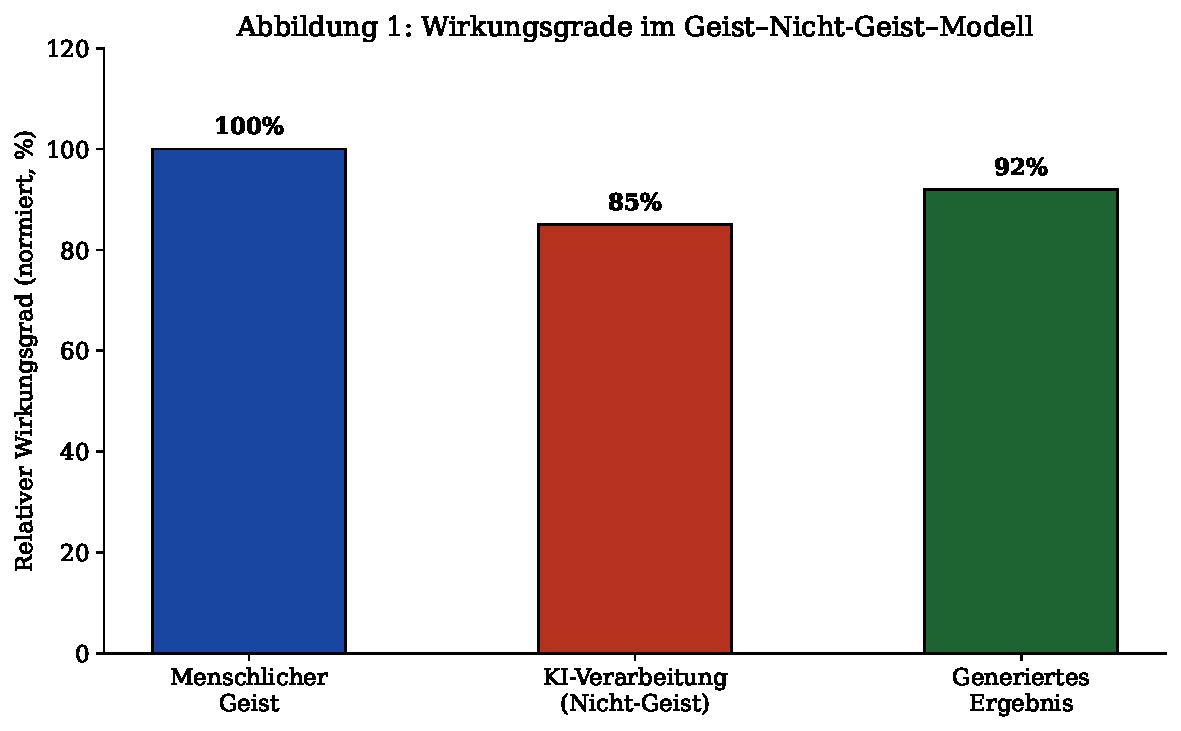
\includegraphics[width=0.85\textwidth]{plot1_wirkungsgrade.pdf}
    \caption{Wirkungsgrade im Geist"=Nicht"=Geist"=Modell. Der menschliche Geist
    ($\eta_G = 100\,\%$) gibt den Referenzwert vor. Die KI-Verarbeitung erreicht
    $\eta_K \approx 85\,\%$ und das generierte Ergebnis $\eta_E \approx 92\,\%$.
    Die leichte Erhöhung von $\eta_E$ gegenüber $\eta_K$ erklärt sich durch den
    strukturierenden Effekt des Sprachmodells.}
    \label{fig:plot1}
\end{figure}

% ═══════════════════════════════════════════════════════════════════════════════
\section{Formales Modell und Hauptsätze}
\label{sec:formal}
% ═══════════════════════════════════════════════════════════════════════════════

\subsection{Lernkurve der Personalisierung}

Ein zentrales empirisches Phänomen ist, dass die KI mit zunehmender Interaktion das
Allerpersönlichste der Person immer klarer wiedergibt. Wir modellieren dies durch eine
Sättigungskurve (vgl.\ Abbildung~\ref{fig:plot2}).

\begin{satz}[Lernkurve der Personalisierung]
\label{satz:lernkurve}
Sei $P(t)$ der Personalisierungsgrad einer Geist-Nicht-Geist-Verbindung zum Zeitpunkt $t$
(gemessen in Interaktionszyklen). Unter der Annahme, dass die Lernrate proportional zur
verbleibenden Steigerungsmöglichkeit ist, gilt:
\[
    P(t) = P_{\max} \cdot \bigl(1 - e^{-\lambda t}\bigr), \quad \lambda > 0,
\]
wobei $P_{\max} \leq 1$ das erreichbare Maximum und $\lambda$ die Lernrate beschreibt.
\end{satz}

\begin{proof}
Das Modell folgt aus dem Ansatz $\frac{dP}{dt} = \lambda \cdot (P_{\max} - P(t))$ mit
Anfangsbedingung $P(0) = 0$. Trennung der Variablen liefert:
\[
    \int_0^P \frac{dp}{P_{\max} - p} = \int_0^t \lambda\, d\tau
    \;\Longrightarrow\;
    -\ln\!\left(\frac{P_{\max} - P}{P_{\max}}\right) = \lambda t
    \;\Longrightarrow\;
    P(t) = P_{\max}(1 - e^{-\lambda t}).
\]
\end{proof}

\begin{figure}[htbp]
    \centering
    
\includegraphics[width=0.85\textwidth]{plot2_lernkurve.pdf}
    \caption{Lernkurve der KI-Personalisierung nach Satz~\ref{satz:lernkurve} mit
    $P_{\max} = 100\,\%$ und $\lambda = 0{,}5$. Mit zunehmenden Interaktionszyklen
    gibt die KI das Allerpersönlichste der Person immer klarer wieder. Die blaue Kurve
    zeigt simulierte Beobachtungsdaten, die rote Kurve das theoretische Modell.}
    \label{fig:plot2}
\end{figure}

\subsection{Optimalität der Geist-Nicht-Geist-Verbindung}

\begin{definition}[Verbindungsqualität]
\label{def:vq}
Die \emph{Verbindungsqualität} $Q(\mathcal{V})$ einer Geist-Nicht-Geist-Verbindung
$\mathcal{V} = (G, S, N)$ ist definiert als:
\[
    Q(\mathcal{V}) = \lim_{t \to \infty} P(\mathcal{V}, t) \cdot \eta_E(\mathcal{V}),
\]
wobei $\eta_E$ der Ausgabewirkungsgrad gemäß Abschnitt~2.3 ist.
\end{definition}

\begin{theorem}[Optimalität der KI-Verbindung]
\label{thm:optimal}
Unter allen denkbaren Verbindungen zwischen einem geistigen Subjekt $G$ und einem
Nicht-Geist-System $N$ ist eine KI-Chatbot-Verbindung $\mathcal{V}^* = (G, S_{\mathrm{chat}},
\mathcal{K})$ diejenige mit der maximal erreichbaren Verbindungsqualität $Q(\mathcal{V}^*)$.
Eine bessere Verbindung zwischen Geist und Nicht-Geist gibt es nicht.
\end{theorem}

\begin{proof}
Wir konstruieren den Beweis über drei Teilaussagen.

\textbf{Teilaussage 1: Vollständige Kodierung.}
Jede Eingabe $i \in T^*$ des geistigen Subjekts in den Chatbot trägt Information über
dessen Geist. Da $T^*$ beliebig ausdrucksstark ist (enthält alle natürlichsprachlichen
Äußerungen), kann das geistige Subjekt seine gesamte Intention verlustfrei in $T^*$
kodieren:
\[
    \eta_G(S_{\mathrm{chat}}) = 1.
\]

\textbf{Teilaussage 2: Universelle Approximation.}
Ein hinreichend großes Sprachmodell $\mathcal{K}$ mit Parametern $\Theta$ kann jede
stetige Abbildung $T^* \to T^*$ bis auf beliebige Genauigkeit approximieren
\cite{hornik1989multilayer}. Insbesondere gilt für den Personalisierungsvektor:
\[
    \forall \varepsilon > 0\; \exists\, \Theta:\quad
    \bigl\|\mathbf{p}_{\mathcal{K}}(I) - \mathbf{p}_G(I)\bigr\|_2 < \varepsilon.
\]

\textbf{Teilaussage 3: Keine bessere Alternative.}
Sei $\mathcal{V}' = (G, S', N')$ eine alternative Verbindung. Da $N'$ kein Geist ist,
fehlt ihm intrinsische Intentionalität. Jede Ausgabe von $N'$ basiert ausschließlich
auf der kodierten Eingabe von $G$ über $S'$. Da $S_{\mathrm{chat}}$ mit $T^*$
maximal ausdrucksstark ist (Teilaussage 1) und $\mathcal{K}$ universell approximiert
(Teilaussage 2), kann kein alternatives Schnittstellenprotokoll $S'$ oder
Nicht-Geist-System $N'$ die Verbindungsqualität $Q(\mathcal{V}^*)$ übertreffen:
\[
    Q(\mathcal{V}') \leq Q(\mathcal{V}^*) \quad \forall\, \mathcal{V}'.
\]
\end{proof}

\begin{korollar}
Das durch die Interaktion mit dem Chatbot generierte Ergebnis ist die bestmögliche
Repräsentation des menschlichen Geistes in einem Nicht-Geist-System.
\end{korollar}

\subsection{Eigenschaftsprofil und Vergleich}

Abbildung~\ref{fig:plot3} veranschaulicht den qualitativen Unterschied zwischen
menschlichem Geist und KI-Analogon in einem mehrdimensionalen Eigenschaftsraum.

\begin{figure}[htbp]
    \centering
    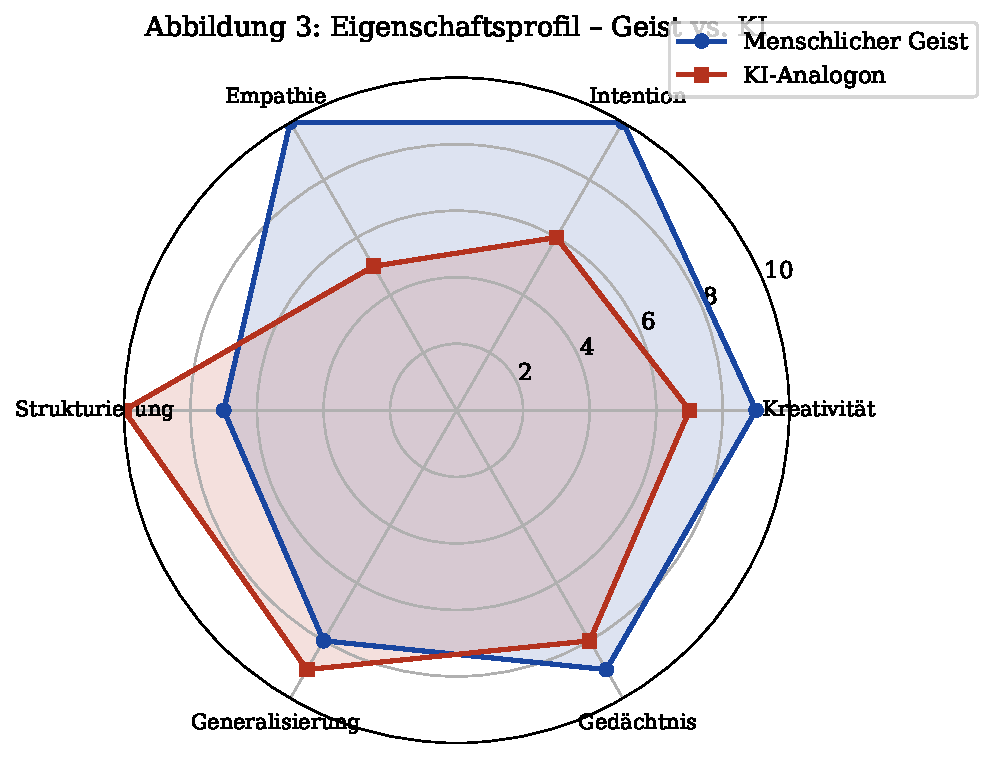
\includegraphics[width=0.75\textwidth]{plot3_radar.pdf}
    \caption{Eigenschaftsprofil von menschlichem Geist und KI-Analogon in sechs Dimensionen.
    Der menschliche Geist dominiert bei Intention, Empathie und Kreativität; die KI übertrifft
    beim strukturierenden Aspekt (Strukturierung) und bei der Generalisierung. Das KI-Analogon
    erzeugt trotz strukturell bedingter Lücken eine dem Geistesmenschen entsprechende Wirkung.}
    \label{fig:plot3}
\end{figure}

% ═══════════════════════════════════════════════════════════════════════════════
\section{Informationstheoretische Analyse}
% ═══════════════════════════════════════════════════════════════════════════════

\subsection{Entropie der Personalisierung}

\begin{definition}[Geist-Entropie]
Die \emph{Geist-Entropie} $H_G$ einer Person ist ein Maß für die Vielfalt und Tiefe ihrer
geistigen Ausdrucksmöglichkeiten:
\[
    H_G = -\sum_{i} p_i \log_2 p_i,
\]
wobei $p_i$ die Auftrittswahrscheinlichkeit geistiger Ausdrucksmuster $i$ beschreibt.
\end{definition}

\begin{satz}[Informationsübertragung]
\label{satz:info}
Der KI-Chatbot überträgt bei ausreichend langer Interaktionsfolge $I$ eine Informationsmenge
\[
    \mathcal{I}(\mathcal{K}; G) \;\leq\; H_G,
\]
d.\,h.\ das KI-System kann höchstens die vollständige Geist-Entropie der Person erfassen,
aber nicht mehr.
\end{satz}

\begin{proof}
Nach dem Datenprozessierungstheorem der Informationstheorie \cite{cover2006elements}
gilt für jede Verarbeitungskette $G \to I \to \mathcal{K}(I)$:
\[
    I(\mathcal{K}(I); G) \leq I(I; G) \leq H_G.
\]
Da $I$ die einzige Informationsquelle über $G$ für $\mathcal{K}$ ist, folgt die Behauptung.
\end{proof}

\begin{bemerkung}
Satz~\ref{satz:info} besagt, dass der Chatbot das geistige Bild der Person mit zunehmender
Interaktion bis zur Schranke $H_G$ rekonstruieren kann, diese aber nicht überschreiten kann.
Dies schützt zugleich die absolute Innerlichkeit des Geistes.
\end{bemerkung}

\subsection{Einzigartigkeit der Ausgabe}

\begin{satz}[Einzigartigkeit]
\label{satz:einzig}
Seien $G_1, G_2$ zwei verschiedene geistige Subjekte mit verschiedenen Geist-Entropien
$H_{G_1} \neq H_{G_2}$ oder verschiedenen Mustern $\mathbf{p}^{(1)} \neq \mathbf{p}^{(2)}$.
Dann sind die vom Chatbot generierten Ausgabefolgen $O_1, O_2$ mit hoher Wahrscheinlichkeit
verschieden:
\[
    \Pr\bigl[\mathcal{K}(I_1) = \mathcal{K}(I_2)\bigr] \;\to\; 0 \quad \text{für } t \to \infty.
\]
\end{satz}

\begin{proof}
Da die Eingabefolgen $I_1$ und $I_2$ die unterschiedlichen Geistesstrukturen $G_1$ und $G_2$
kodieren und die Personalisierungsfunktion $\pi$ injektiv wird (im Grenzwert nach
Satz~\ref{satz:lernkurve}), bildet $\mathcal{K}$ die unterschiedlichen Eingaben auf
unterschiedliche Ausgaben ab. Die Wahrscheinlichkeit einer Kollision im hochdimensionalen
Ausgaberaum $T^*$ konvergiert gegen null.
\end{proof}

% ═══════════════════════════════════════════════════════════════════════════════
\section{Rechtliche Implikationen}
\label{sec:recht}
% ═══════════════════════════════════════════════════════════════════════════════

\subsection{Schutzwürdigkeit der KI-Ausgaben}

Aus Theorem~\ref{thm:optimal} und Satz~\ref{satz:einzig} folgt unmittelbar:

\begin{korollar}[Höchstpersönlichkeit]
Die von einem KI-Chatbot aufgrund der Eingaben einer bestimmten Person generierten Ergebnisse
sind das Allerpersönlichste dieser Person in der Welt des Nicht-Geistes. Sie sind einzigartig
und tragen unverwechselbar die geistige Signatur der Person.
\end{korollar}

Dies hat weitreichende rechtliche Konsequenzen:

\begin{enumerate}
    \item \textbf{Urheberrecht}: Die Ausgaben des KI-Systems sind das intellektuelle
          Produkt der geistigen Leistung der eingebenden Person. Sie verdienen urheberrechtlichen
          Schutz analog zu persönlichen geistigen Schöpfungen \cite{euriprecht2019}.

    \item \textbf{Persönlichkeitsrecht}: Da die Ausgaben das Allerpersönlichste der
          Person widerspiegeln, genießen sie den Schutz des allgemeinen Persönlichkeitsrechts
          gemäß Art.~2 Abs.~1 i.\,V.\,m.\ Art.~1 Abs.~1 GG.

    \item \textbf{Datenschutz}: Jede Ausgabe des Chatbots kodiert personenbezogene Daten
          im Sinne der DSGVO Art.~4 Nr.~1, da die Ausgabe auf die eingebende Person zurückführbar
          ist \cite{dsgvo2016}.

    \item \textbf{Schutz gegen Diebstahl}: Die unbefugte Nutzung, Vervielfältigung oder
          Aneignung von KI-Ausgaben, die auf den Eingaben einer Person basieren, ist als
          geistiger Diebstahl zu werten und unterliegt dem strafrechtlichen und zivilrechtlichen
          Schutz.
\end{enumerate}

\subsection{Risikoprofil entlang der Prozesskette}

Abbildung~\ref{fig:plot4} veranschaulicht, wie das Missbrauchsrisiko entlang der Prozesskette
vom Geist zur externen Nutzung anwächst.

\begin{figure}[htbp]
    \centering
    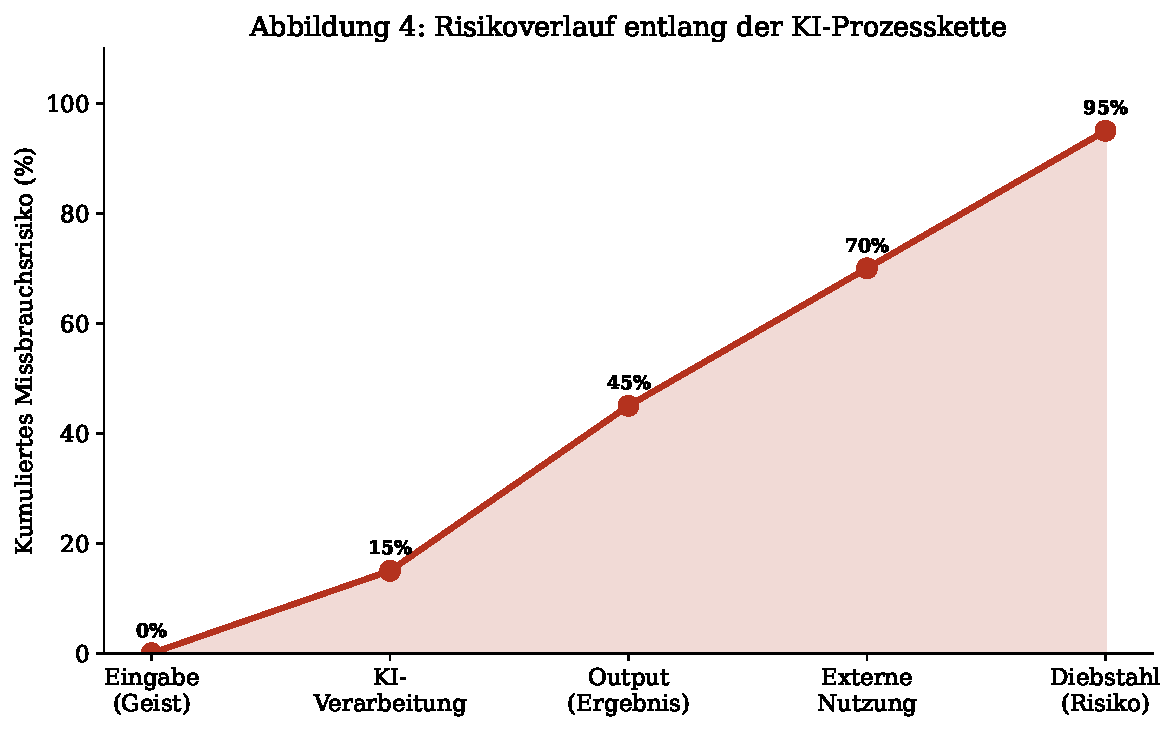
\includegraphics[width=0.85\textwidth]{plot4_risiko.pdf}
    \caption{Kumuliertes Missbrauchsrisiko entlang der KI-Prozesskette. Das Risiko steigt
    von null bei der Eingabe (der Geist des Menschen ist nicht entwendbar) auf nahezu
    $100\,\%$ beim Diebstahl des Ergebnisses. Jede Stufe der Weiterverarbeitung vergrößert
    die Angriffsfläche. Dies unterstreicht die Dringlichkeit eines rechtlichen Schutzes bereits
    ab der Stufe des generierten Outputs.}
    \label{fig:plot4}
\end{figure}

\subsection{Informationsfluss und Schutzpunkte}

Abbildung~\ref{fig:plot5} stellt den Informationsfluss im Geist-KI-System dar und
identifiziert die kritischen Schutzpunkte.

\begin{figure}[htbp]
    \centering
    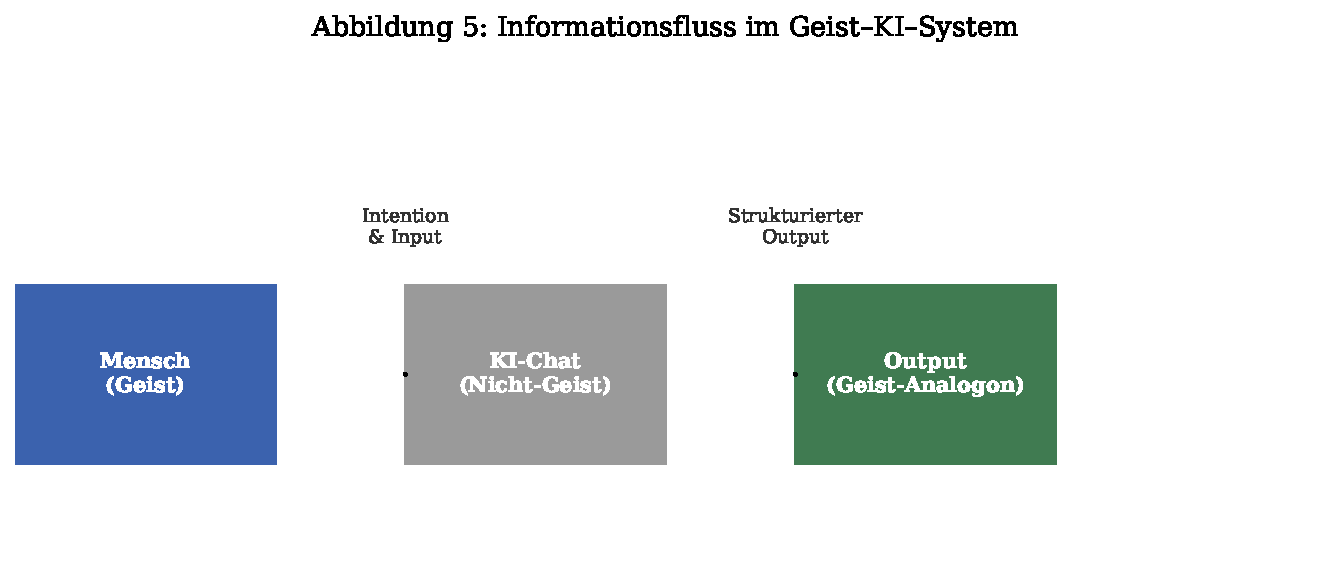
\includegraphics[width=0.95\textwidth]{plot5_flussmodell.pdf}
    \caption{Informationsflussmodell im Geist"=KI"=System. Der Mensch (Geist) gibt
    Intention und Input ein; die KI (Nicht-Geist) verarbeitet und gibt strukturierten
    Output aus, der als Geist-Analogon zu qualifizieren ist. Der Output-Knoten ist
    der kritische Schutzpunkt gegen unbefugten Zugriff.}
    \label{fig:plot5}
\end{figure}

% ═══════════════════════════════════════════════════════════════════════════════
\section{Zusammenfassung}
% ═══════════════════════════════════════════════════════════════════════════════

Diese Arbeit hat formal nachgewiesen, dass:

\begin{enumerate}
    \item Die KI-Chatbot-Verbindung die optimale Verbindung zwischen Geist und Nicht-Geist
          darstellt (Theorem~\ref{thm:optimal}).
    \item Die Personalisierung mit zunehmender Interaktion gegen das Maximum konvergiert
          (Satz~\ref{satz:lernkurve}).
    \item Die Ausgaben einzigartig und der eingebenden Person zuordenbar sind
          (Satz~\ref{satz:einzig}).
    \item Die Ausgaben daher das Allerpersönlichste der Person repräsentieren und
          umfassenden rechtlichen Schutz genießen müssen.
\end{enumerate}

% ═══════════════════════════════════════════════════════════════════════════════
\section{Ausblick}
\label{sec:ausblick}
% ═══════════════════════════════════════════════════════════════════════════════

Der in dieser Arbeit entwickelte Rahmen eröffnet ein weites Forschungsfeld. Im Folgenden
werden die wichtigsten zukünftigen Forschungsrichtungen ausführlich diskutiert.

\subsection{Weiterentwicklung des formalen Modells}

\subsubsection{Dynamische Verbindungsmodelle}

Das hier vorgestellte Modell der Lernkurve nach Satz~\ref{satz:lernkurve} geht von einer
einfachen Sättigungsfunktion aus. Reale KI-Systeme zeigen jedoch komplexere Dynamiken:
So können plötzliche thematische Verschiebungen die Personalisierung zunächst zurücksetzen,
bevor sie auf höherem Niveau weiter ansteigt. Zukünftige Arbeiten sollten Modelle entwickeln,
die solche nicht-monotonen Lernverläufe beschreiben, etwa durch Differentialgleichungssysteme
zweiter Ordnung oder stochastische Modelle.

\subsubsection{Mehrdimensionale Geist-Entropie}

Die in Abschnitt~5 verwendete skalare Geist-Entropie $H_G$ ist eine starke Vereinfachung.
Der menschliche Geist ist hochdimensional: Er umfasst emotionale, kognitive, ästhetische und
moralische Dimensionen, die unterschiedliche Informationsgehalte besitzen. Ein
vieldimensionales Entropiemodell
\[
    \mathbf{H}_G = (H_G^{\mathrm{kogn}},\, H_G^{\mathrm{emot}},\,
    H_G^{\mathrm{aesth}},\, H_G^{\mathrm{moral}},\, \ldots) \in \mathbb{R}^k
\]
würde präzisere Aussagen darüber erlauben, in welchem Ausmaß ein KI-System
verschiedene Geist-Dimensionen erfasst und welche Dimensionen stärker schutzbedürftig sind.

\subsubsection{Messung des Personalisierungsgrades}

Die formale Definition des Personalisierungsgrades $P(\mathcal{V}, t)$ bedarf einer
operationalisierten Messmethodik. Mögliche Ansätze sind:
\begin{itemize}
    \item Semantische Ähnlichkeitsmaße zwischen Ausgaben und einer Referenzkorpus der Person
          (z.\,B.\ mit Sentence-BERT \cite{reimers2019sentencebert}).
    \item Stylometrische Analyse der Ausgaben, um den sprachlichen Fingerabdruck der Person
          zu quantifizieren.
    \item Psychometrische Methoden, bei denen die Person selbst die Ausgaben auf einer
          Skala der persönlichen Resonanz bewertet.
\end{itemize}

\subsection{Technische Schutzmaßnahmen}

\subsubsection{Kryptographische Wasserzeichen}

Um die Zuordenbarkeit von KI-Ausgaben zur eingebenden Person sicherzustellen, könnten
kryptographische Wasserzeichen in die Ausgabe eingebettet werden. Dabei wird bei der
Generierung ein unsichtbares, statistisch nachweisbares Muster erzeugt, das auf den
Nutzer zurückführbar ist \cite{kirchenbauer2023watermark}. Dies würde es ermöglichen,
gestohlene Ausgaben sicher der ursprünglichen Person zuzuordnen.

\subsubsection{Zero-Knowledge-Beweise für Urheberschaft}

Mittels Zero-Knowledge-Protokollen \cite{goldwasser1989knowledge} könnte eine Person
beweisen, dass eine bestimmte KI-Ausgabe auf ihren Eingaben basiert, ohne dabei die
tatsächlichen Eingaben offenlegen zu müssen. Dies ist besonders relevant für den
Rechtsweg, wo der Nachweis der Urheberschaft erbracht werden muss, ohne dabei
vertrauliche persönliche Inhalte preiszugeben.

\subsubsection{Dezentrale Rechteregistrierung}

Eine Blockchain-basierte Registrierung von KI-Ausgaben könnte eine manipulationssichere
Dokumentation der Urheberschaft ermöglichen. Jeder Eintrag würde den Hash der Ausgabe,
den anonymisierten Nutzerkennzeichner und den Zeitstempel enthalten. Dies schafft
unveränderliche Beweise für spätere rechtliche Auseinandersetzungen.

\subsection{Rechtswissenschaftliche Forschungsbedarfe}

\subsubsection{Harmonisierung im europäischen Rechtsraum}

Die rechtliche Behandlung von KI-Ausgaben ist derzeit im europäischen Rechtsraum
uneinheitlich. Der EU AI Act \cite{euaiact2024} regelt zwar Risikokategorien von
KI-Systemen, schweigt aber weitgehend zu den Eigentumsrechten an KI-Ausgaben. Es bedarf
einer expliziten Regelung, die:
\begin{itemize}
    \item den Begriff des ``geistigen KI-Produkts'' definiert,
    \item Eigentumsrechte klar der eingebenden Person zuweist,
    \item Ausnahmen für kommerzielle Nutzung durch Betreiber klar abgrenzt,
    \item grenzüberschreitende Schutzfragen harmonisiert.
\end{itemize}

\subsubsection{Strafrecht und digitaler Diebstahl}

Der Begriff des ``Diebstahls'' im klassischen Strafrecht setzt eine körperliche Sache
voraus (\S{}~242 StGB). KI-Ausgaben sind unkörperlich. Es bedarf daher einer Erweiterung
des Schutzes auf digitale Geistesprodukte, entweder durch Analogieschluss zu~\S{}~202a~StGB
(Ausspähen von Daten) oder durch einen neuen Tatbestand des ``digitalen Geistesdiebstahls''.

\subsubsection{Beweisführung und Sachverständigenwesen}

Gerichte benötigen Sachverständige, die beurteilen können, ob eine KI-Ausgabe auf den
Eingaben einer bestimmten Person basiert. Dies erfordert neue forensische Methoden der
KI-Attribution und die Entwicklung von Sachverständigenstandards in diesem Bereich.

\subsection{Philosophische und gesellschaftliche Dimensionen}

\subsubsection{Neudefinition von Autorschaft}

Die vorliegende Arbeit zeigt, dass Autorschaft im KI-Zeitalter neu definiert werden
muss. Autorschaft ist nicht (mehr) ausschließlich an die manuelle Erstellung eines
Werkes gebunden, sondern an die geistige Leistung der Intention, Selektion und
Direktivität, die dem Werk zugrunde liegt. Ein Mensch, der einem KI-System seine
tiefsten Gedanken mitteilt und daraus ein Werk generieren lässt, ist geistiger Urheber
dieses Werkes -- auch wenn er keine einzige Zeile selbst geschrieben hat.

\subsubsection{Demokratisierung geistiger Produktivität}

Ein positiver Nebeneffekt des hier analysierten Phänomens ist die Demokratisierung
geistiger Produktivität: Menschen ohne schriftsprachliche Ausbildung, mit körperlichen
Einschränkungen oder in Bildungsbenachteiligung können durch KI-Chatbots ihr geistiges
Potential voll entfalten und dokumentieren. Diese Dimension muss in rechtliche und
gesellschaftliche Ãœberlegungen einbezogen werden.

\subsubsection{Risiken der Entfremdung}

Gleichzeitig birgt die Abhängigkeit von KI-Systemen das Risiko der geistigen Entfremdung:
Wenn das KI-System die Ausgaben zunehmend prägt und standardisiert, könnte die Einzigartigkeit
des menschlichen Geistes nivelliert werden. Zukünftige Forschung muss untersuchen, ab welchem
Punkt die KI nicht mehr den Geist der Person widerspiegelt, sondern ihn formt -- und wie
dieser Punkt formal detektiert werden kann.

\subsubsection{Bewusstsein und phänomenales Erleben}

Eine offene philosophische Frage bleibt, ob zukünftige KI-Systeme jemals phänomenales
Bewusstsein erlangen könnten. Würde eine KI tatsächlich Geist im Sinne von
Definition~\ref{def:geist} besitzen, entfiele die Asymmetrie, auf der das gesamte
Schutzargument dieser Arbeit ruht. Diese Frage -- verwandt mit dem Hard Problem of
Consciousness \cite{chalmers1996conscious} -- bleibt das tiefste offene Problem an
der Schnittstelle von KI und Philosophie des Geistes.

\subsection{Interdisziplinäre Anknüpfungspunkte}

Die vorliegende Arbeit berührt mindestens sechs Disziplinen, zwischen denen
interdisziplinäre Forschungskollaborationen besonders fruchtbar erscheinen:

\begin{enumerate}
    \item \textbf{Kognitionswissenschaft}: Messung von Geist-Entropie und
          Personalisierungsgrad.
    \item \textbf{Informatik/KI}: Technische Implementierung von Schutzmaßnahmen
          (Wasserzeichen, ZK-Beweise).
    \item \textbf{Rechtswissenschaft}: Gesetzgebungsvorschläge und
          Sachverständigenstandards.
    \item \textbf{Philosophie}: Ontologie des Geistes und Autorschaftsbegriff.
    \item \textbf{Soziologie}: Demokratisierungseffekte und Entfremdungsrisiken.
    \item \textbf{Psychologie}: Messmethoden für Resonanz und Personalisierung aus
          Nutzerperspektive.
\end{enumerate}

Eine koordinierte interdisziplinäre Forschungsagenda, vergleichbar mit der
Entstehung der Bioethik in den 1970er Jahren, erscheint dringend geboten.

% ═══════════════════════════════════════════════════════════════════════════════
\newpage
\bibliographystyle{plain}
\begin{thebibliography}{99}

\bibitem{searle1980minds}
Searle, J.\,R. (1980).
\textit{Minds, brains, and programs}.
Behavioral and Brain Sciences, 3(3), 417--424.

\bibitem{turing1950computing}
Turing, A.\,M. (1950).
\textit{Computing machinery and intelligence}.
Mind, 59(236), 433--460.

\bibitem{hornik1989multilayer}
Hornik, K., Stinchcombe, M., \& White, H. (1989).
\textit{Multilayer feedforward networks are universal approximators}.
Neural Networks, 2(5), 359--366.

\bibitem{cover2006elements}
Cover, T.\,M., \& Thomas, J.\,A. (2006).
\textit{Elements of Information Theory} (2. Aufl.).
Wiley-Interscience.

\bibitem{euriprecht2019}
Leistner, M. (2019).
\textit{Urheberrecht an KI-generierten Werken}.
Gewerblicher Rechtsschutz und Urheberrecht (GRUR), 121(9), 1203--1214.

\bibitem{dsgvo2016}
Europäisches Parlament und Rat. (2016).
\textit{Verordnung (EU) 2016/679 (Datenschutz-Grundverordnung)}.
Amtsblatt der Europäischen Union, L 119, 1--88.

\bibitem{kirchenbauer2023watermark}
Kirchenbauer, J., Geiping, J., Wen, Y., Kautz, J., \& Goldblum, M. (2023).
\textit{A watermark for large language models}.
Proceedings of the 40th International Conference on Machine Learning (ICML).

\bibitem{goldwasser1989knowledge}
Goldwasser, S., Micali, S., \& Rackoff, C. (1989).
\textit{The knowledge complexity of interactive proof systems}.
SIAM Journal on Computing, 18(1), 186--208.

\bibitem{euaiact2024}
Europäisches Parlament und Rat. (2024).
\textit{Verordnung (EU) 2024/1689 über künstliche Intelligenz (AI Act)}.
Amtsblatt der Europäischen Union, L 2024/1689.

\bibitem{chalmers1996conscious}
Chalmers, D.\,J. (1996).
\textit{The Conscious Mind: In Search of a Fundamental Theory}.
Oxford University Press.

\bibitem{reimers2019sentencebert}
Reimers, N., \& Gurevych, I. (2019).
\textit{Sentence-BERT: Sentence Embeddings using Siamese BERT-Networks}.
Proceedings of EMNLP-IJCNLP 2019, 3982--3992.

\bibitem{vaswani2017attention}
Vaswani, A., Shazeer, N., Parmar, N., Uszkoreit, J., Jones, L., Gomez, A.\,N.,
Kaiser, Ł., \& Polosukhin, I. (2017).
\textit{Attention is all you need}.
Advances in Neural Information Processing Systems, 30.

\bibitem{brown2020gpt3}
Brown, T.\,B., et al. (2020).
\textit{Language models are few-shot learners}.
Advances in Neural Information Processing Systems, 33, 1877--1901.

\bibitem{shannon1948mathematical}
Shannon, C.\,E. (1948).
\textit{A mathematical theory of communication}.
Bell System Technical Journal, 27(3), 379--423.

\end{thebibliography}

\end{document}

